\subsection{Diagrammes UML}

\subsubsection{Diagramme du module Hex et Awalé}

Le diagramme suivant représente les classes et les fonctions du module Hex et du module Awalé.
Il montre les classes \texttt{HexBoard} et \texttt{AwaleBoard} qui représentent les plateaux de jeu
du Hex et de l'Awalé, ainsi que les fonctions pour l'implémentation des différents algorithmes de jeu.
Il contient également les classes d'exceptions pour gérer les erreurs et les exceptions dans le jeu.

\begin{figure}[!htb]
    \centering
    \fbox{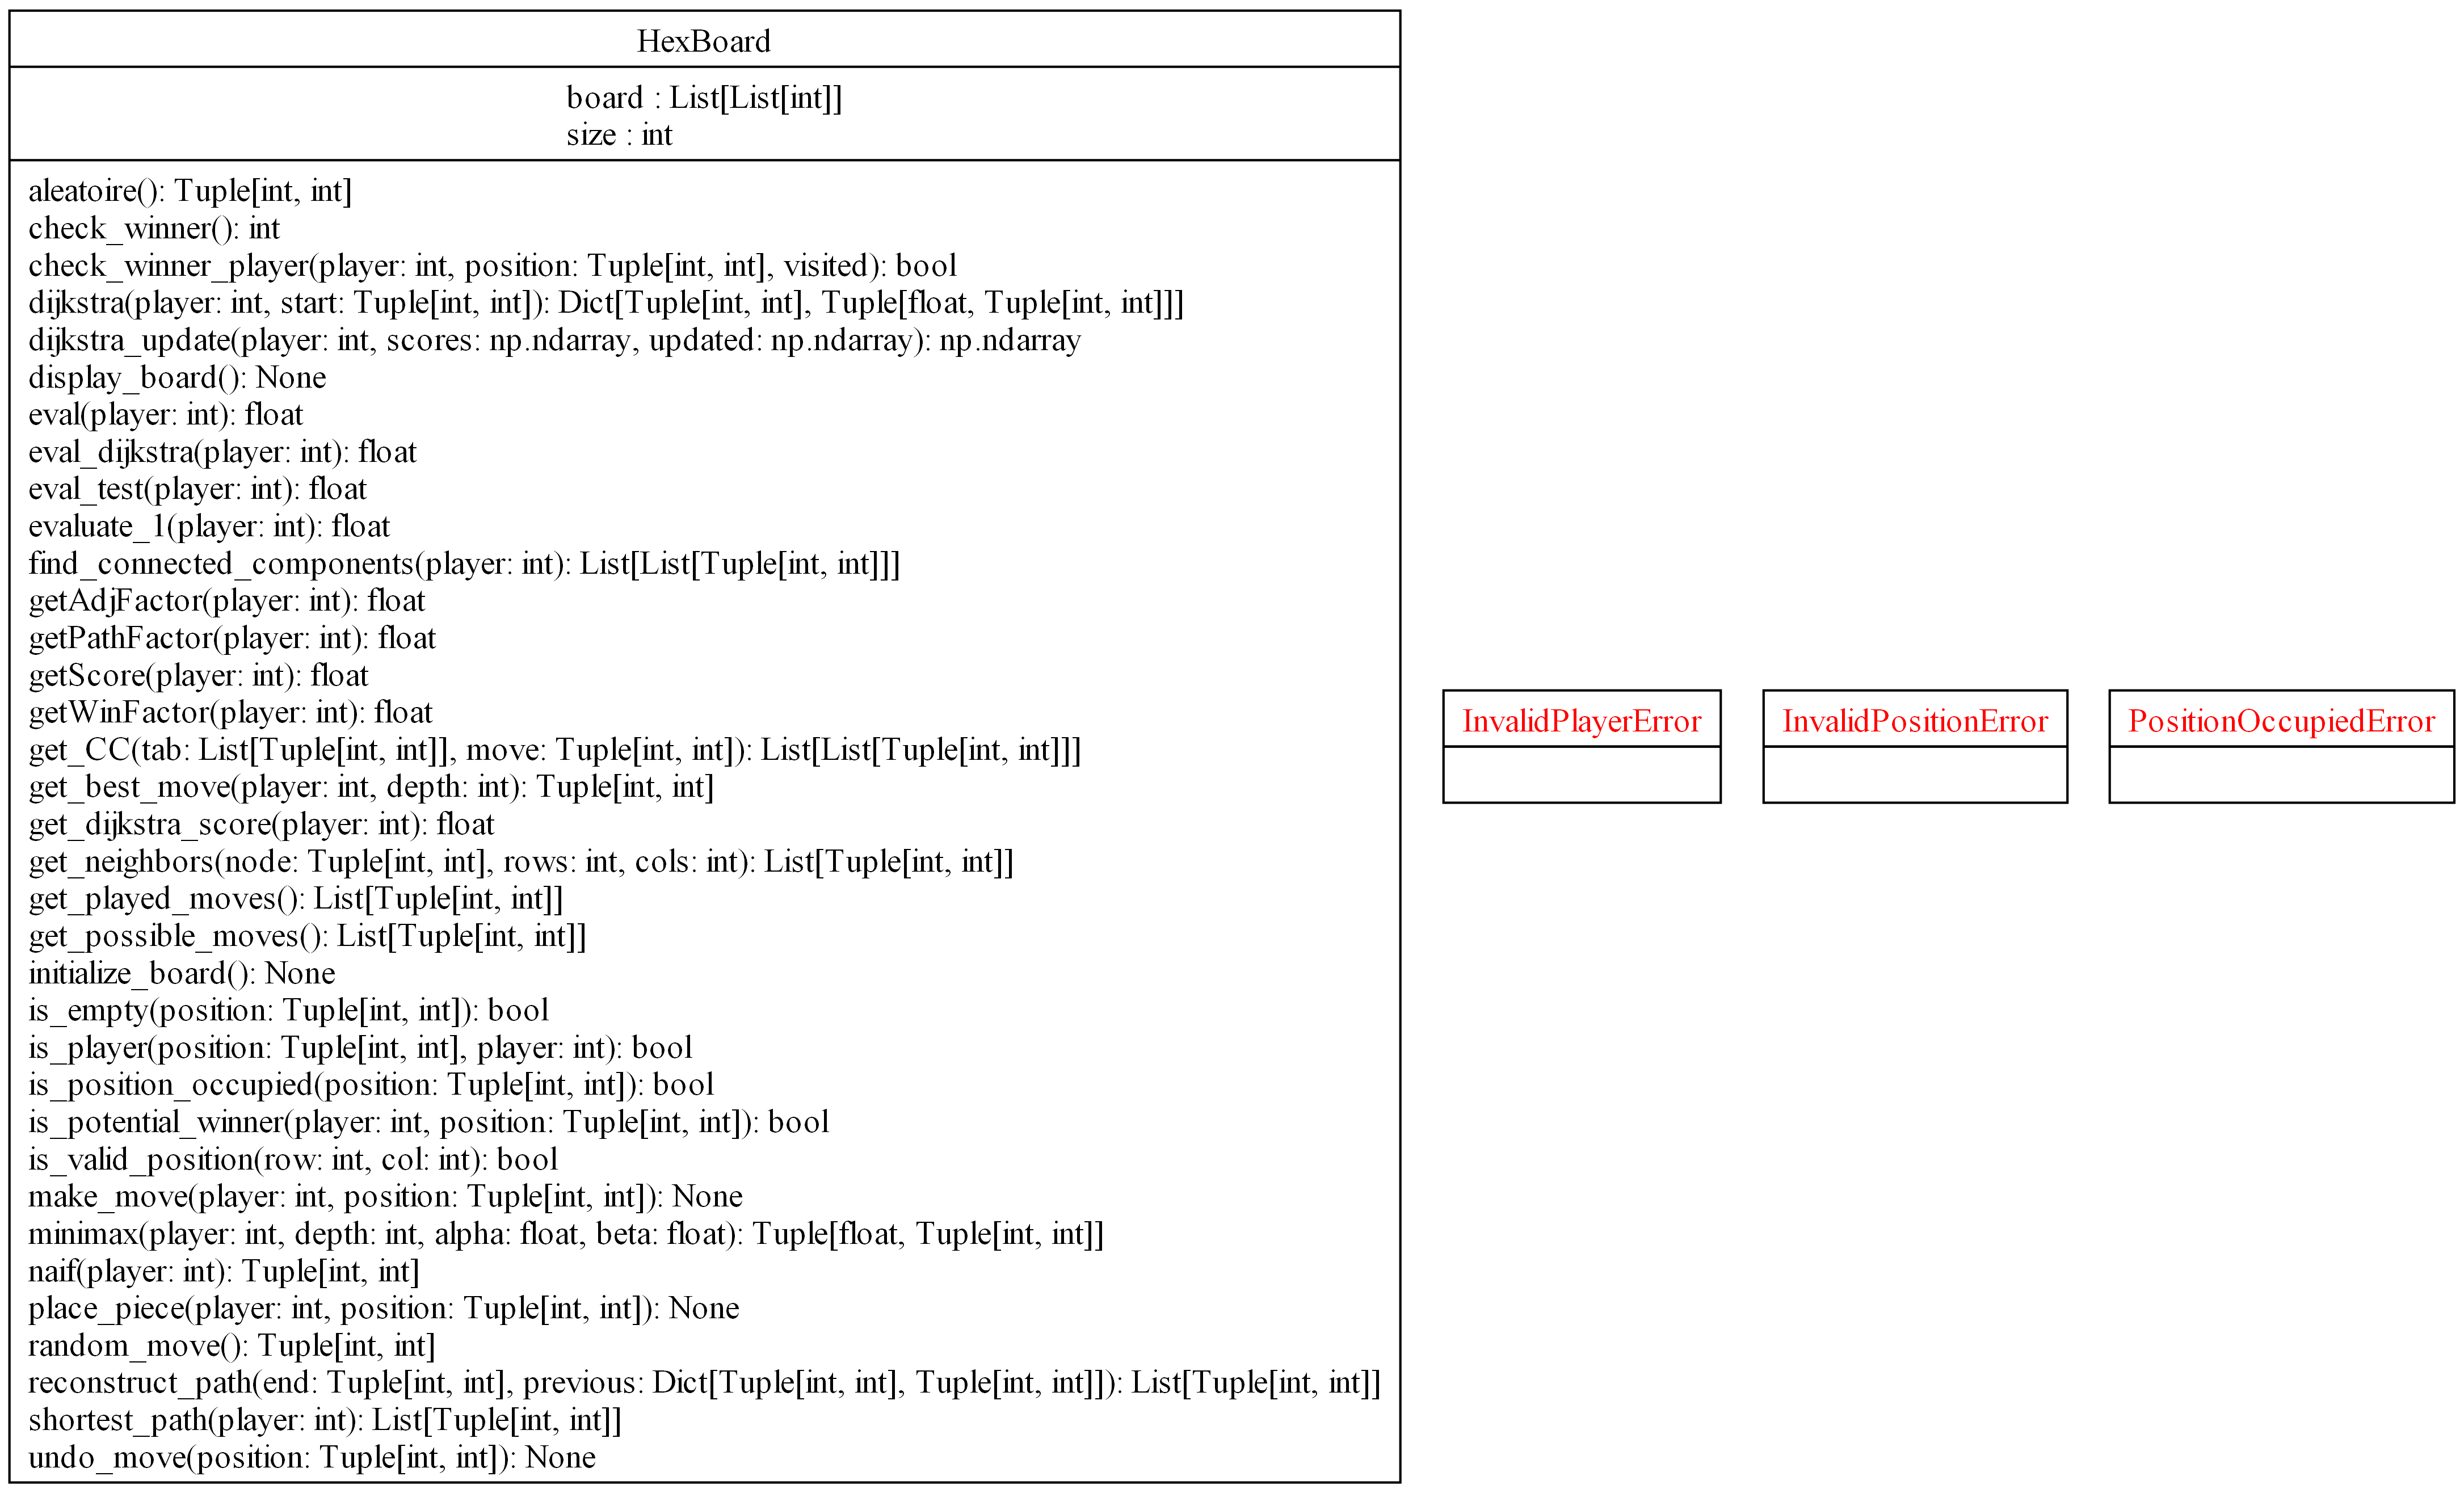
\includegraphics[width=.8\linewidth]{root/UML_hex.png}}
    \caption{Diagramme UML du module Hex}\label{Fig:UML_hex}
\end{figure}
\begin{figure}[!htb]
    \centering
    \fbox{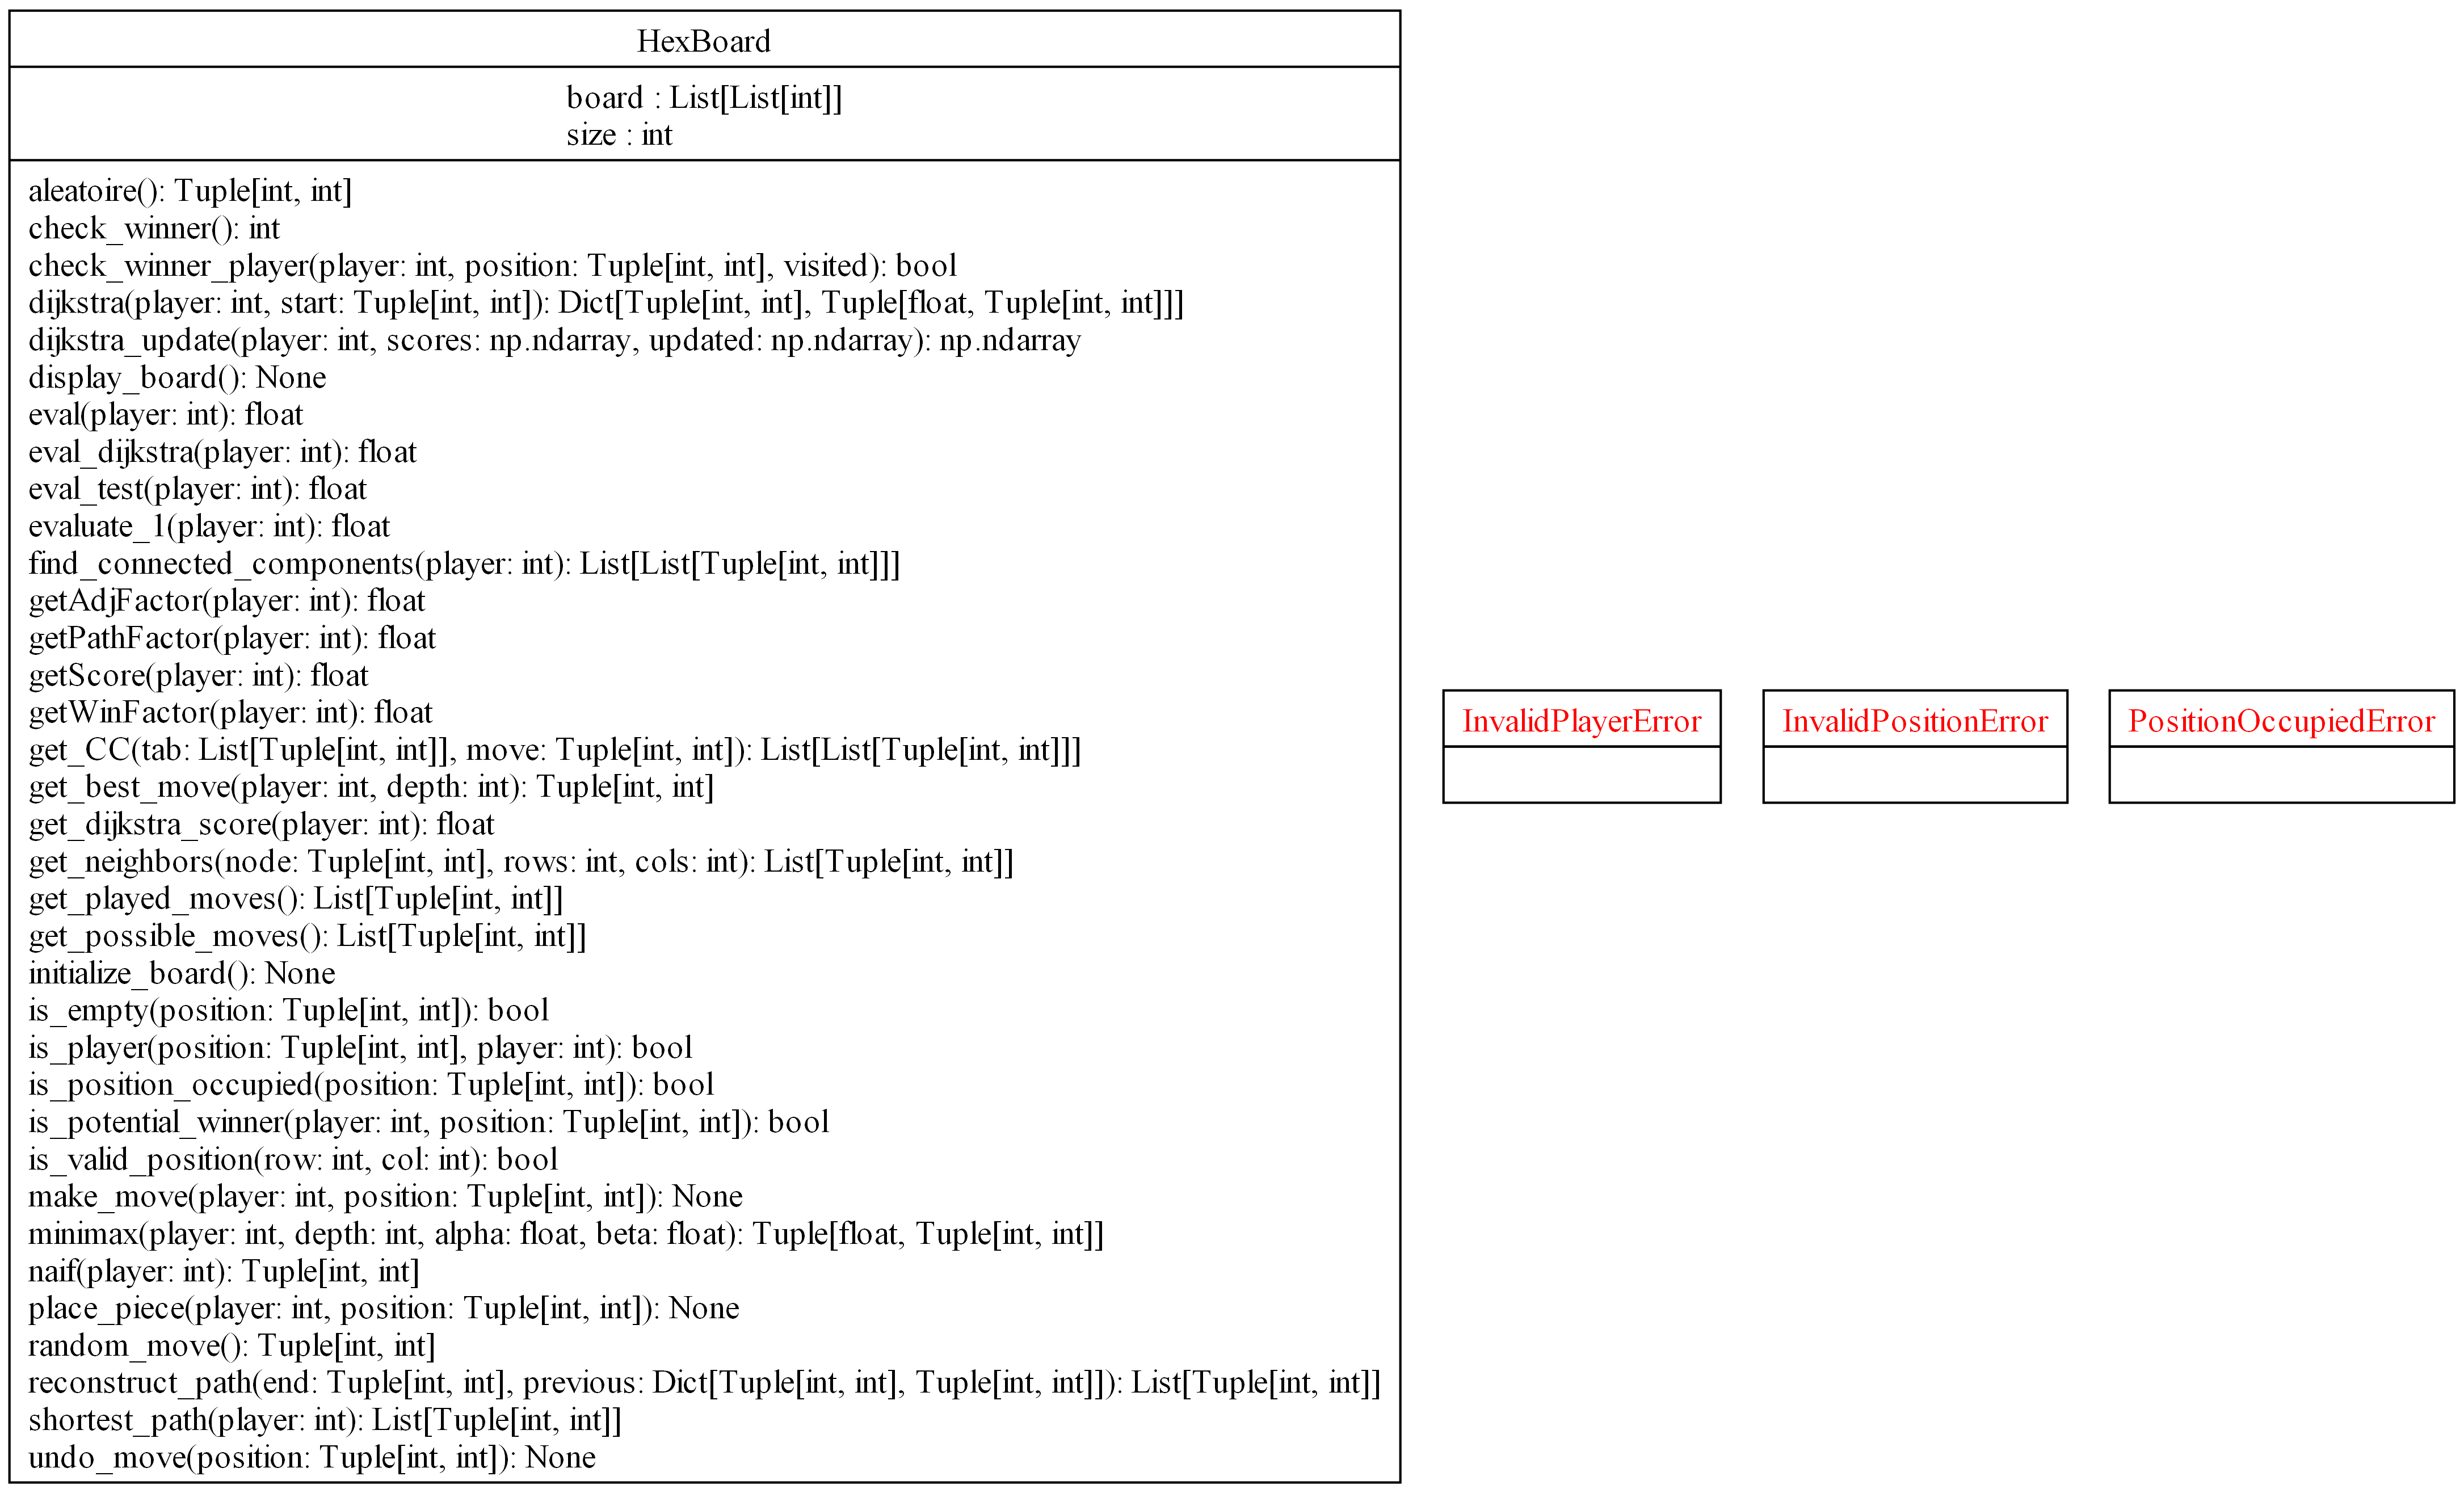
\includegraphics[width=.8\linewidth]{root/UML_hex.png}}
    \caption{Diagramme UML du module Hex}\label{Fig:UML_hex}
\end{figure}

Ces diagrammes UML ont pû être générés automatiquement à partir du code source grâce à 
`pyreverse' qui est un outil de génération de diagrammes UML pour Python.

\subsubsection{Diagramme de fonctionnement de l'application}

Le diagramme suivant représente le fonctionnement de l'application. Il montre les différentes
classes et fonctions de l'application, ainsi que les interactions entre elles.
Il montre comment l'interface graphique communique avec les modules de jeu pour afficher
le plateau de jeu et les coups joués par les joueurs. Les détails ne sont pas affichés
pour des raisons de lisibilité, de même que seul le module Hex est représenté en détail.

\begin{figure}[!htb]
    \centering
    \fbox{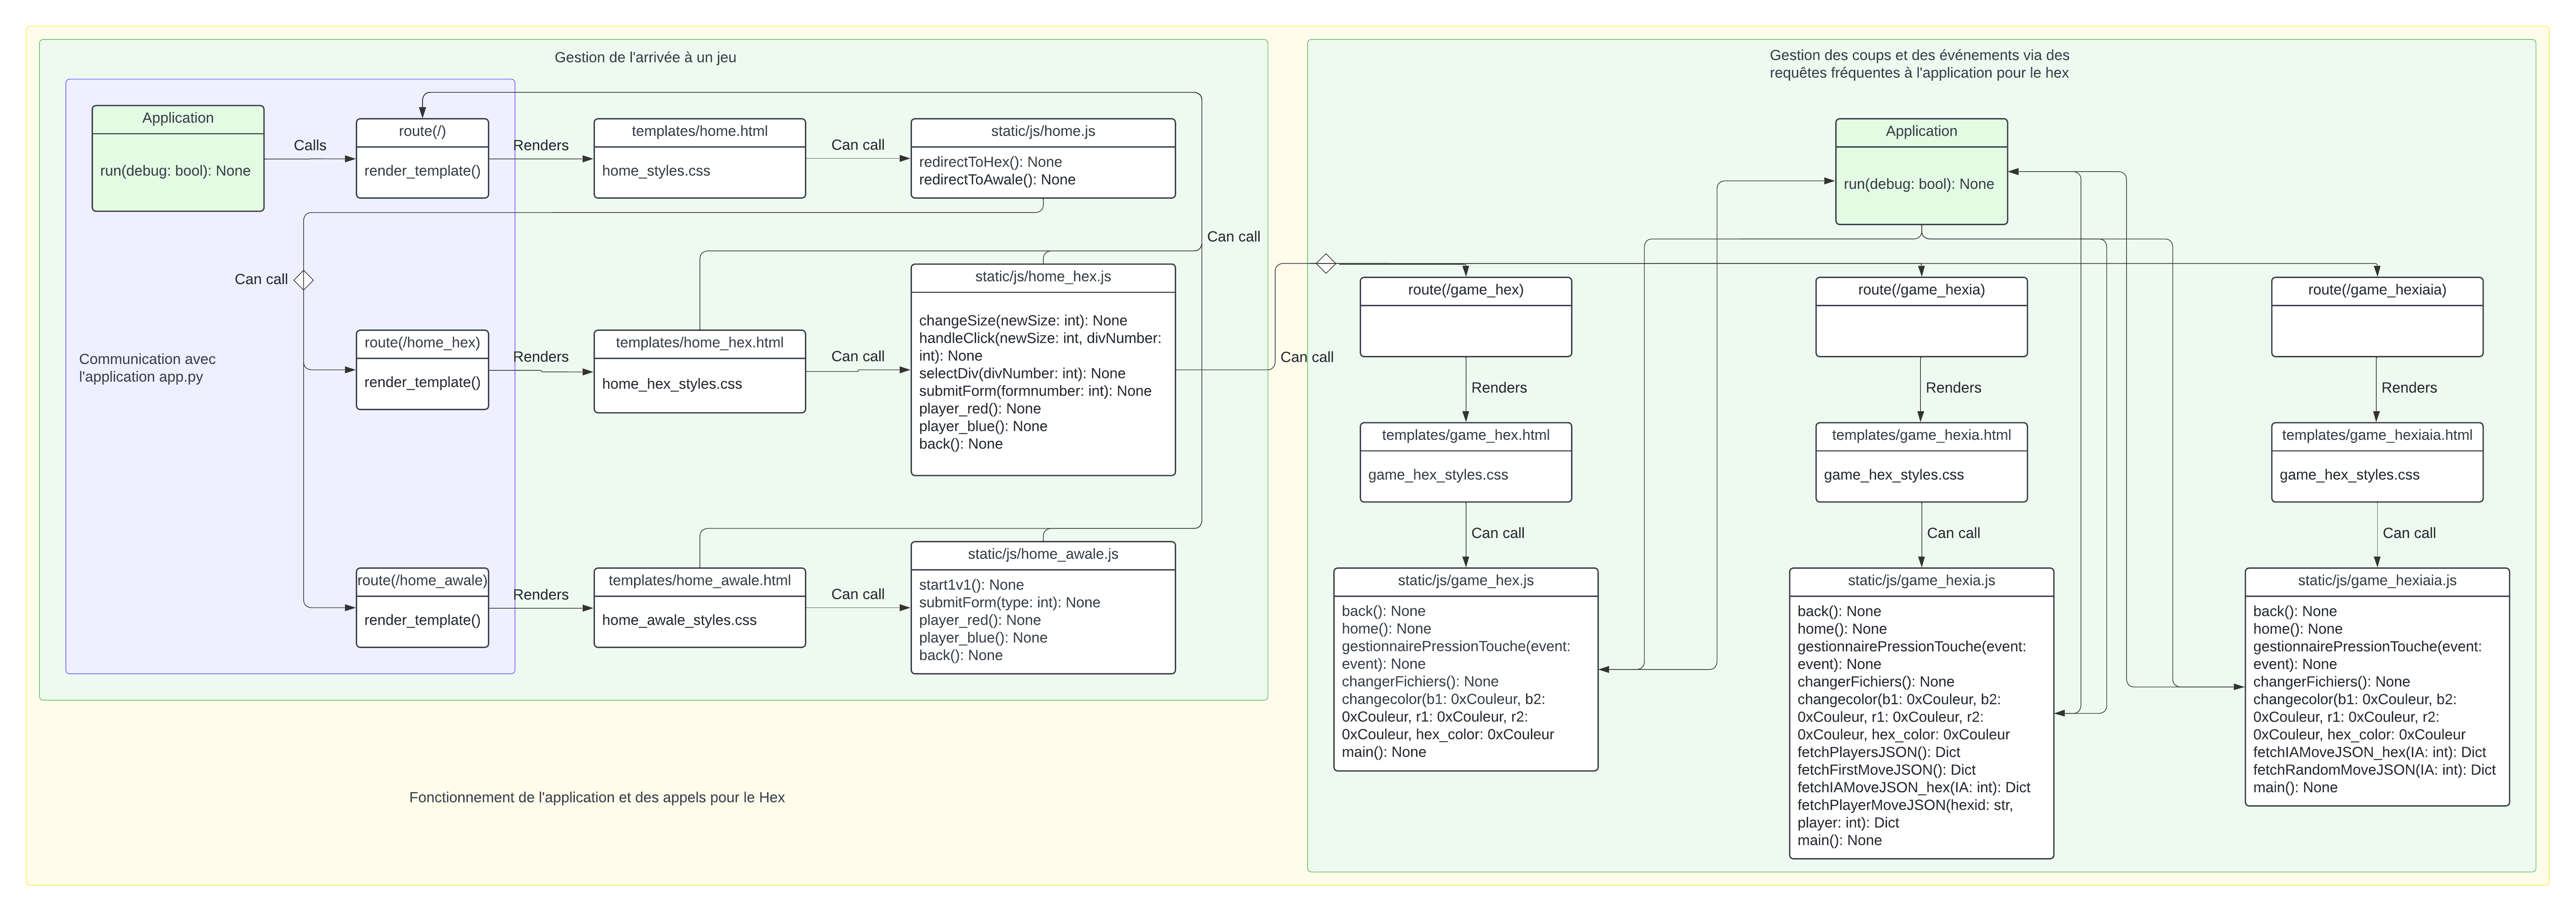
\includegraphics[width=\linewidth]{root/UML_app.png}}
    \caption{Diagramme UML de l'application}\label{Fig:UML_app}
\end{figure}

